\documentclass{article}
\usepackage{ctexcap}
\usepackage{amsmath,amsthm, amsfonts, amssymb, array}
\usepackage{graphicx,booktabs,xcolor}
\usepackage{hyperref}
\usepackage{fancybox,fancyhdr, geometry}
\usepackage{subfigure}
\usepackage[toc,page]{appendix}

%%%% 让图片链接直接到图片,而不是标题
\usepackage{caption}
\captionsetup{hypcap=true}


%%%% 设置页边距
\geometry{left=3cm,right=3cm,top=2.5cm,bottom=2.5cm}
\newcommand{\bc}[1]{\textbf{{\color{blue}#1}}}
\newcommand{\PreserveBackslash}[1]{\let\temp=\\#1\let\\=\temp}
\newcolumntype{C}[1]{>{\PreserveBackslash\centering}p{#1}}
\newcolumntype{R}[1]{>{\PreserveBackslash\raggedleft}p{#1}}
\newcolumntype{L}[1]{>{\PreserveBackslash\raggedright}p{#1}}
%\makeatletter
%\renewcommand\tableofcontents{%
%    \section*{{\centering\rule{\textwidth}{0.5pt}\\[1ex]\contentsname\\[0.8ex]\rule{\textwidth}{0.5pt}}
%        \@mkboth{%
%           \MakeUppercase\contentsname}{\MakeUppercase\contentsname}}%
%    \@starttoc{toc}}
%\makeatother
\pagestyle{fancy}
\lhead{\zihao{-5}{\textit{统计之都}~~http://cos.name}}
\chead{}
\rhead{\zihao{-5}{\textit{一道抛硬币问题的不同解法和比较}}} % 要改写
\lfoot{}
\cfoot{\thepage}
\rfoot{}

%\renewcommand{\contentsname}{目录}
%\renewcommand{\refname}{参考文献}
%\renewcommand{\abstractname}{摘要}
\renewcommand{\figurename}{\heiti\small 图}
\renewcommand{\tablename}{\heiti\small 表}
%\renewcommand{\appendixname}{附录}
%\renewcommand{\appendixtocname}{附录}
%\renewcommand{\appendixpagename}{附录}

\setlength{\belowcaptionskip}{2pt plus 1pt minus 1pt}
\setlength{\abovecaptionskip}{2pt plus 1pt minus 1pt}

\begin{document}


%\thispagestyle{empty}
%\tableofcontents
%\setcounter{chapter}{5}
%\setcounter{section}{-1}
\title{\heiti 一道抛硬币问题的不同解法和比较\thanks{在线阅读:\url{http://cos.name/2011/01/different-ways-to-solve-a-tossing-problem/}} }
\author{魏太云\thanks{邮箱:weitaiyun@gmail.com;主页:\url{taiyun.cos.name};单位:中国人民大学统计学院.}}
%
\date{}
\maketitle

%\setcounter{page}{1}
\addcontentsline{toc}{section}{摘要}%
\begin{abstract}
\noindent{\hspace{2em}本文针对求指定花样在抛硬币时首次出现时间期望的问题,分别从统计模拟、马氏过程、延迟更新过程、鞅、
随机图等角度出发对该类问题进行了模拟和理论方面的解答,并展现了各种方法的特点和实用价值.}\\

{\heiti 关键词:}  古典概率\quad  统计模拟\quad 马氏过程\quad  延迟更新过程\quad 鞅 \quad 随机图\quad GERT
\end{abstract}

%\tableofcontents

\section{问题背景}
一道古典概率题目:一个均匀硬币,反复抛掷,请问一直抛到出现HTT(正反反)和HTH(正反正)的期望次数分别是多少?

首先考虑一下HTT和HTH的首达时刻的期望是否相同,很容易犯的一个错误是认为HTT和HTH的出现没本质区别,因此它们的首达时刻的期望也是一样的.
但实际上它们是有区别的.一个具体解释如下,在当前时刻得到HT的时候:
\begin{itemize}
\item 针对HTT目标:如果下一次抛出T,则成功得到HTT序列;
如果下次抛出结果为H,则得不到HTT序列,但刚抛出的H是HTT的首字母,为之后得到HTT序列奠定了部分基础.
\item 针对HTH目标:如果下一次抛出H,则成功得到HTH序列;
如果下次抛出结果为T,则得不到HTH序列,且刚抛出的T并不是HTH的首字母,也就说之后需要完全“从头开始”.
\end{itemize}

因此,HTT的首达时间期望应该比HTH要小,这和大多数人的第一直观(或者说错觉)是不一致的.此外,首次得到HTT和HTH的区别可以通过分析它们的
随机图(图\ref{fig:htt} 和图\ref{fig:hth})更直观地得到.

\section{统计模拟}
该问题看似很简单,但用传统的古典方法计算时,发现非常繁琐.
考虑到古典方法的困难性,采用数值模拟来计算该问题,在R中编写函数来模拟该问题,分别模拟
10000次,发现HTT和HTH的首达时间的期望分别近似为8和10,代码(来自\cite{3})和运行结
果如下.
\begin{small}
\begin{verbatim}
coin.seq = function(v) {
    x = NULL
    n = 0
    while (!identical(x, v)) {
        x = append(x[length(x) - 1:0], rbinom(1, 1, 0.5))
        n = n + 1
    }
    return(n)
}
> mean(htt <- replicate(1e+05, coin.seq(c(1, 0, 0)))) ## HTT模拟均值
[1] 8.00304
> mean(hth <- replicate(1e+05, coin.seq(c(1, 0, 1)))) ## HTH模拟均值
[1] 10.0062
\end{verbatim}
\end{small}

显然,模拟的结果是HTT和HTH的首达时间明显不同,画出10000次模拟下它们的箱线图(如图\ref{fig:coin}).
\begin{figure}[btp]
\centering
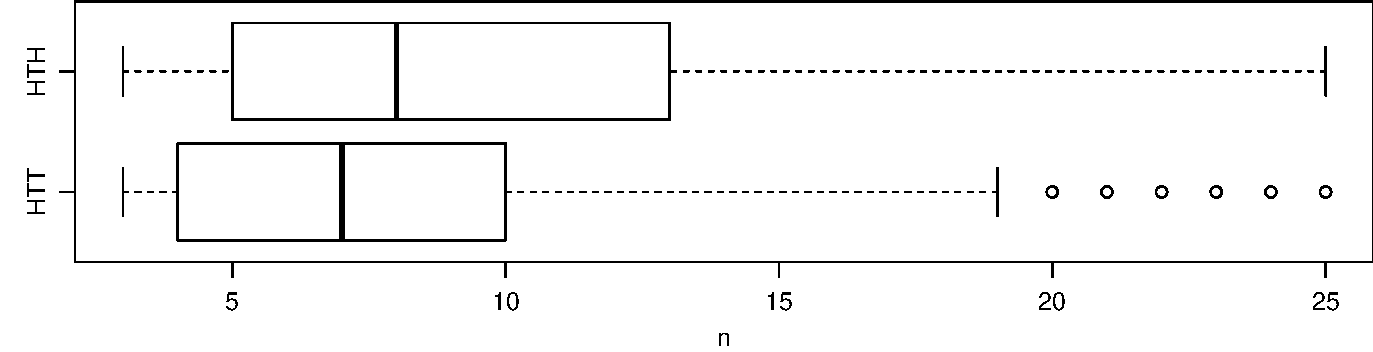
\includegraphics[width=14cm]{coin.pdf}
\caption{10000次模拟下HTT和HTH首达时刻的箱线图(来自\cite{3})}\label{fig:coin}
\end{figure}

此外,HTT和HTH的首达时间在$10000$次统计模拟情况下非常接近于8和10,而它们的理论值具体应该是多少就不是数值模拟能解决的了.下面借助其他工具来精确求解该问题及其拓展问题.



\section{马氏过程}
可以借鉴马氏过程的思路, 先求HTT首次出现时间的期望$E(N_\text{HTT})$:每一步扔下去是否到达HTT仅和前两步有关,
所以已知前两步状态,后面的期望步数就确定了,
那么假设前两步是HT,TH,HH,TT之后的到达HTT所需步数为$x_1,x_2,x_3,x_4$,那么就可以列出方程组(\ref{eq:markov-HTT}).
\begin{equation}\label{eq:markov-HTT}
\left\{
\begin{array}{rrrrrr}
x_1&=&0.5&+&0.5(x_2+1)\\
x_2&=&0.5(x_3+1)&+&0.5(x_1+1)\\
x_3&=&0.5(x_3+1)&+&0.5(x_1+1)\\
x_4&=&0.5(x_2+1)&+&0.5(x_4+1)\\
\end{array}\right.
\end{equation}


方程组(\ref{eq:markov-HTT})中,第一个式子意思是,HT之后一步如果扔的是T,那么就终止,1步到达HTT,如果扔的是H,那么回到TH的状态,
也就是$x_2$.其他三个式子以此类推,
求解方程组(\ref{eq:markov-HTT}),得$x_1=4, x_2=6, x_3=6, x_4=8$,于是.
$$E(N_\text{HTT})=0.25(x_1+x_2+x_3+x_4)+2=8$$

即HTT首次出现时间的期望为8.

同理,求HTH首次出现时间的期望$E(N_\text{HTH})$,列出方程组(\ref{eq:markov-HTH})


\begin{equation}\label{eq:markov-HTH}
\left\{
\begin{array}{rrrrrr}
x_1&=&0.5&+&0.5(x_4+1)\\
x_2&=&0.5(x_3+1)&+&0.5(x_1+1)\\
x_3&=&0.5(x_3+1)&+&0.5(x_1+1)\\
x_4&=&0.5(x_2+1)&+&0.5(x_4+1)\\
\end{array}\right.
\end{equation}

求解方程组(\ref{eq:markov-HTH}),得$x_1=6, x_2=8, x_3=8, x_4=10$,于是.
$$E(N_\text{HTH})=0.25(x_1+x_2+x_3+x_4)+2=10$$

即HTH首次出现时间的期望为10.

如此一来,一道本来非常繁琐的题目就可以通过马氏链的思想轻松解决了.但是该方法在状态长度较大时(比如求HTHTTH)的时候比较麻烦,
后面将要介绍的延迟更新过程和鞅理论可以更便捷地解决这一问题.
\section{延迟更新过程}
设$\{X_n, n=1,2,\cdots\}$为一列独立非负随机变量,$X_1$具有分布$G$,而$X_n$具有分布$F$,$n \geqslant 2$. 令$S_0=0$, $S_n=\sum\limits_{i=1}^n X_i$,$n  \geqslant 1$,且定义

\begin{equation}\label{eq:renew}
N_D(t)=\sup\{n:S_n \leqslant t\}
\end{equation}
则随机过程$\{N_D(t), t\geqslant0\}$称为延迟更新过程\cite{1}.

记首次更新时间的分布为花样(比如抛硬币中的HTT、HTH等)首次发生时间的分布,而后面的间隔分布为该花样复制之间的时间分布,以$N(n)$记到时刻$n$发生花样的次数,
则$\{N(n), n \geqslant 1\}$是一个延迟更新过程.

令$p_i, i= 1,2,\cdots,k$表示$k$叠(即花样长度为$k$)花样中各个元素的单次概率,由延迟更新过程的强大数定律和布莱克威尔定理可知
\begin{equation}\label{eq:timeE}
E(\text{花样之间的时间})=(\prod_{i=1}^k p_i)^{-1}
\end{equation}

从式(\ref{eq:timeE})中可以知道花样之间时间的期望值,比如抛掷均匀硬币时,第$n$次出现HHH和第$n+1$次$(n \geqslant 1)$出现HHH的
间隔时间的期望就是$1/0.5^3=8$.下面我们以两次花样间隔时间的期望作为桥梁来求首次出现花样时间的期望.

首先计算HTT首次出现时间的期望,我们发现在HTT出现后,下一次重现HTT和这一次的HTT完全无关,也就是说本次的HTT不能为下一步的HTT
提供任何基础,因此两次HTT的间隔时间期望就等于HTT 首次出现时间的期望,即$E(N_\text{HTT})=8$.

然后再计算HTH首次出现时间的期望,和HTT不同的是HTH出现之后能为下一次出现HTH提供基础比如再抛掷出TH后,结合上一次最后的花样元素H,
即可得到下一次的HTH.为了计算HTH首次出现时间的期望,我们需要做的就是剥离这种基础.

用全概率公式,将得到HTH后再次得到HTH的事件一分为二,分别是接着抛出TH和没有抛出TH,对应的分别是“有基础”和“没有基础”的两种情况,
如果抛出TH,则$2$步到达下一个HTH,如果抛不出,设期望为$X$.根据全概率公式得
\begin{equation}\label{eq:TH}
\begin{array}{rl}
  &E(\text{花样之间的时间})\\
  =&P(\text{下两次抛出TH})\cdot 2 + P(\text{下两次未抛出TH})\cdot X\\
  =&(1/4)\cdot 2 + (3/4) X
  =8
\end{array}
\end{equation}

求解式(\ref{eq:TH}),得到$N_\text{HTH|!TH}=X=10$(其中!TH表示未抛出TH),即在前两次未抛出TH情况下,得到HTH的时间期望为$10$.
无论是首次更新(对应分布$G$)还是之后的更新(对应分布$F$),$N_\text{HTH|!TH}$都等于$10$.

现计算前两次抛出TH时,得到HTH的时间期望(不能利用前面基础),如果接下来两步抛出TH(概率为$1/4$),那么$4$步达到HTH,如果抛不出
TH(概率为$3/4$),那么期望转为$2+N_\text{HTH|!TH}$次,根据全概率公式得
\begin{equation}
  N_\text{HTH|TH}=\frac{1}{4}4 + \frac{3}{4}(2+N_\text{HTH|!TH})=1+9=10
\end{equation}

至此,可以计算出首次抛出HTH的平均时间了.
\begin{equation}
  N_\text{HTH}=N_\text{HTH|TH}+N_\text{HTH|!TH}=\frac{1}{4}10 + \frac{3}{4}10=10
\end{equation}

对任意有限离散分布,都可以用该方法类似地求其花样首次出现时间的期望.

\section{鞅}
通过构造鞅可以计算任意有限离散分布下各种花样首次出现时间的期望,本节的关键也就是构造鞅,并且是构造一个非常巧妙的鞅.

以\cite{1}中的例子来演示鞅的构造:假设序贯地观察一列独立同分布的离散随机变量,一天一个,直到某个给定的序列出现.
设每次观察的结果分别以概率$1/2,1/3,1/6$
分别取为$0,1,2$ ,我们希望求直到游程$020$ 出现为止的平均时间$N$.

\begin{table}[ht]
\centering
\scriptsize{
\caption{首达时间为$N$时的赌博情况\label{tab:020}}
\begin{tabular}{r|C{0.75cm}C{0.75cm}C{0.75cm}C{0.75cm}C{0.75cm}C{0.75cm}C{0.75cm}C{0.75cm}C{0.75cm}}
  \hline
天数 & 1 & 2 & 3 &  4 &  5 & $\cdots$ & $N-2$ & $N-1$ & $N$ \\
  \hline
实际情况 &  &  &  &  &  &  &   0 &   2 &   0 \\
\hline
赌徒1的赌法 &   0 &   2 &   0 &  &  &  &  &  &  \\
赌徒2的赌法 &  &   0 &   2 &   0 &  &  &  &  &  \\
赌徒3的赌法 &  &  &   0 &   2 &   0 &  &  &  &  \\
$\cdots$ &  &  &  &  &  &  &  &  &  \\
赌徒$N-2$的赌法 &  &  &  &  &  &  &  \bc{0} &   \bc{2} &   \bc{0} \\
赌徒$N-1$的赌法 &  &  &  &  &  &  &  &   0 &   2 \\
赌徒$N$的赌法 &  &  &  &  &  &  &  &  &   \bc{0} \\
   \hline
\end{tabular}}
\end{table}

为了计算$E(N)$. 设想有一列赌徒在一个公平的赌场参赌,每人起初都
有$1$元.第$i$ 个赌徒在第$i$天的开始赌起,以他的$1$元打赌那天的观察值将是
$0$ .如果他赢了(从而他有$1/2^{-1}=2$ 元),就以$2$ 元打赌下一个结果是$2$ .如果这次赢
了(从而他有$1/(2^{-1} \times6^{-1})=12$ 元) ,就以全部$12$ 元打赌下一个结果是$0$ .因此每个赌徒如果
在三次打赌中输掉任何二次,将输$1$ 元,但三次都赢了将赢$1/(2^{-1}\times2^{-1}\times6^{-1})-1=23$ 元.每天一开
始又一个赌徒开始赌.记 $X_n$为第n 天结束时赌场的总赢得.由于所有的打
赌都是公平的,故得$\{X_n, n\geqslant 1\}$是鞅,均值为$0$ .

以$N$记直到序列$020$ 出现的时间,如表 \ref{tab:020} 所示(表中蓝色粗体字为\textbf{恰好完全匹配}的赌博).
故在第$N$ 天结束时赌徒$1,..., N-3$ 都输$1$元,赌徒$N-2$ 赢了
$23$元,赌徒$N-1$输$1$元(因为第$N-1,N$ 天的观察结果是$2,0$,与该赌徒的答案不能匹配),
赌徒$N$ 赢$1$元(因为第$N$ 天的观察结果是$0$,恰好匹配). 所以
$$
X_N=N-3-\big((\frac{1}{2} \times \frac{1}{2}\times \frac{1}{6})^{-1} - 1\big) - \big((\frac{1}{2})^{-1} - 1\big) - 1=N-26$$

又由于$E(X_N)=0$,故$E(N)=26$,即得到$020$的首次时间的期望为$26$.

该方法具有很强的通用性,通过表 \ref{tab:020} 可以看出,该方法仅需看最后$k$($k$为花色长度)个赌徒和指定花色的匹配情况,具体来说,对任意$k$叠的花样,其首次出现时间的期望是
\begin{equation}\label{eq:martingale}
N_k = \sum_{i=1}^k f_i \frac{1}{p_{1}\cdots p_{i}}
\end{equation}

其中,$f_i$为$0-1$变量,表示花样中前$i$个元素构成的序列是否和后$i$个元素构成的序列完全一致;若一致,取1,若不完全一致,取0.
$p_i$表示花样中第$i$个元素的单次概率.

根据式(\ref{eq:martingale}),可以很方便地编程计算任意有限离散分布下各种花样首次出现时间的期望.R程序(Mathematica程序见\cite{4})如下:


\begin{small}
\begin{verbatim}
coinE <- function(res.seq, p.seq){
    E <- 1/prod(p.seq)
    n <- length(res.seq)
    for(i in 1:(n-1)){
        f <- 1*!sum(abs(diff(res.seq,i)))
        if(f==1) E <- E + 1/prod(p.seq[1:(n-i)])
    }
    return(E)
}
\end{verbatim}
\end{small}

\verb|res.seq|是输入花样,需用整数表示;\verb|p.seq|和\verb|res.seq|等长,表示对应花样元素的单次概率.
用该程序计算HTT和HTH的首次发生时间期望,得到期望值分别为8、10.

\begin{small}
\begin{verbatim}
> coinE (c(1,0,0), rep(0.5,3)) ## HTT首次发生时间期望
[1] 8
> coinE (c(1,0,1), rep(0.5,3)) ## HTH首次发生时间期望
[1] 10
\end{verbatim}
\end{small}

当然,还可以计算更复杂的例子,比如

\begin{small}
\begin{verbatim}
> ## 抛掷均匀骰子,得到123456123456首次时间期望
> coinE (c(1:6,1:6), rep(1/6,12))
[1] 2176828992
> ## 抛掷不均匀硬币(正反面概率分别为0.4,0.6),得到HTHTHTHT首次时间期望
> coinE (rep(1:2,4), rep(c(0.4,0.6),4))
[1] 395.2739
\end{verbatim}
\end{small}

花色信息及随机变量分布见上面程序中的注释(\verb|##|后面的文字).

\section{GERT方法}
GERT方法(Graph Evaluation and Review Technique)是解决随机网络问题中的一种方法,它结合了流线图理论
、矩母函数、计划评审技术等多种方法.文献\cite{2}较为详细地介绍了该方法,并利用GERT解答了本文开头提出的问题.
GERT方法的优势是可以解决更复杂、更一般的问题,并得到更一般的结论.这里仅仅给出该方法的结论.

图 \ref{fig:htt} 和图 \ref{fig:hth} 分别是实现HTT和HTH的随即网络图($p=q=0.5$,用$Z$对每次抛掷硬币做标记).


结合梅森公式,可使用GRET方法得到HTT和HTH的首达时刻的期望分别是8和10,并且可以得到抛掷$n$次得到HTT和HTH的概率,如
式(\ref{eq:gert1})和(\ref{eq:gert2}).
%\begin{equation}\label{eq:gert}
%  \begin{array}{rcl}
%  P_\text{HTT}& = &\sum\limits_{j=0}^{[(n-3)/3]} {n-2j-3 \choose j}(-1)^j (\frac{1}{2})^{3j+3}\\
%  P_\text{HTH}& = &\sum\limits_{j=0}^{[(n-3)/3]} \sum\limits_{k=0}^j {n+k-2j-3\choose j} {j \choose k} (-1)^j(\frac{1}{2})^{3j+3}\\
%\end{array}
%\end{equation}

\begin{align}
\label{eq:gert1}
P_\text{HTT}& = \sum_{j=0}^{[(n-3)/3]} {n-2j-3 \choose j}(-1)^j (\frac{1}{2})^{3j+3}\\
\label{eq:gert2}
P_\text{HTH}& = \sum_{j=0}^{[(n-3)/3]} \sum_{k=0}^j {n+k-2j-3\choose j} {j \choose k} (-1)^j(\frac{1}{2})^{3j+3}
\end{align}


\begin{figure}[h]
\centering
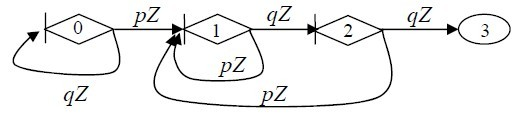
\includegraphics[width=8cm]{HTT}
\caption{实现HTT 的随机网络图(来自文献\cite{2})}\label{fig:htt}
\end{figure}

\begin{figure}[h]
\centering
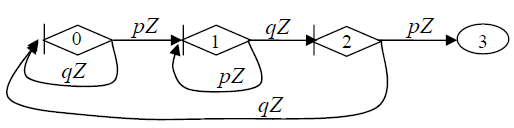
\includegraphics[width=8cm]{HTH}
\caption{实现HTH 的随机网络图(来自文献\cite{2})}\label{fig:hth}
\end{figure}

该方法的细节情况可以在文献\cite{2}中得到,此处不表.
\section{总结}
本文用统计模拟、马氏过程、延迟更新过程、鞅、GERT等各种角度求解了抛掷硬币时,HTT和HTH的首次到达时间的期望.得到的结论有

\begin{itemize}
\item 统计模拟最为直观简便,不需要太多理论,非常实用,但不能得到精确值,并且在花样长度较长时,需要花费很长时间求得一个近似程度较高的解.
\item 借助马氏过程的转移概率的概念,可以求出期望的精确值,但在花样长度增加时,需要计算的方程数目呈指数速度增长($2^n$),不方便求解.
\item 延迟更新过程和鞅方法都能直观、快速求出期望的精确值(尤其是鞅方法),并且可以拓广到任意离散分布下的任意有限长度花样,计算速度很快.
\item GERT方法虽然显得较为复杂,但是可以得到更多信息,并且可以更系统地解决更广泛的与随机图相关的问题.
\end{itemize}

本文所涉及的题目是最常见的抛硬币问题,但通过该题目的多种方法求解和相互比较可以获得很多有意思的东西,
显示了随机过程中这些工具的实用价值.

现代概率论和随机过程中很多知识都可以以抛硬币等初级问题来展开引入,因此关注这些初级问题或许并不仅仅是纯粹的无聊游戏;当然,做这些
题目也可以当做是纯粹的陶冶情操,锻炼思维.

\addcontentsline{toc}{section}{致谢}%
\section*{致谢}
感谢阿杜兄的热情鼓励、对鞅和延迟更新过程理论的介绍及相关资料的推荐,感谢张景肖老师、贺诗源、高涛、肖楠、魏瑶、陈道铨、韩帅、李曾同学的意见和讨论,
感谢COS主站和论坛上相关文章、帖子及其精彩的回复.

最后,感谢我的导师张波先生,他对我的各种鼓励、各种关怀和各种指导一直是我信心的源泉和前进的动力.
\addcontentsline{toc}{section}{参考文献}%
\begin{thebibliography}{99}
\bibitem{1} Sheldon M Ross. Stochastic Processes. 2nd edition. Wiley Publisher. 1995-01. ISBN: 0471120626.
\bibitem{2} 刘飞燕. 用GERT方法求解两个抛硬币问题. 统计之都. 2009-09. URL: \url{http://cos.name/2009/09/introduction-and-application-of-gert/}.
\bibitem{3} Yihui Xie. Counterintuitive Results in Flipping Coins.
URL: \url{http://yihui.name/en/2009/08/counterintuitive-results-in-flipping-coins/}.
\bibitem{4} 杜传龙. 沽名钓誉一回--- 也谈抛硬币问题. 统计之都.  URL: \url{http://cos.name/cn/topic/16880}
\end{thebibliography}


%\begin{appendices}
%\section{怡轩}
%\end{appendices}

\end{document} 